The performance impact of using \gls{JIT} compilation with Numba on top of Numpy
is illustrated in figure (\ref{fig:3_1_numba}). Here we benchmark the performance
of an implementation of insertion sort, an algorithm with an asymptotic complexity
bound of $O(N^2)$, when using an implementation built with Numpy containers and
compare this to an implementation using JIT compilation on top of Numpy containers.
Both functions are run five times on different inputs of the same size
in figure (\ref{fig:3_1_numba}). On larger problems it becomes apparent
that Numba offers an approximately constant speedup over Numpy, in fact for
sorting arrays of $10^4$ integers the JIT compiled function is $1050 \pm 80$
times faster, where the error is provided to (1 s.f) than the pure Numpy function.

\begin{figure}[!h]
    \centering

  {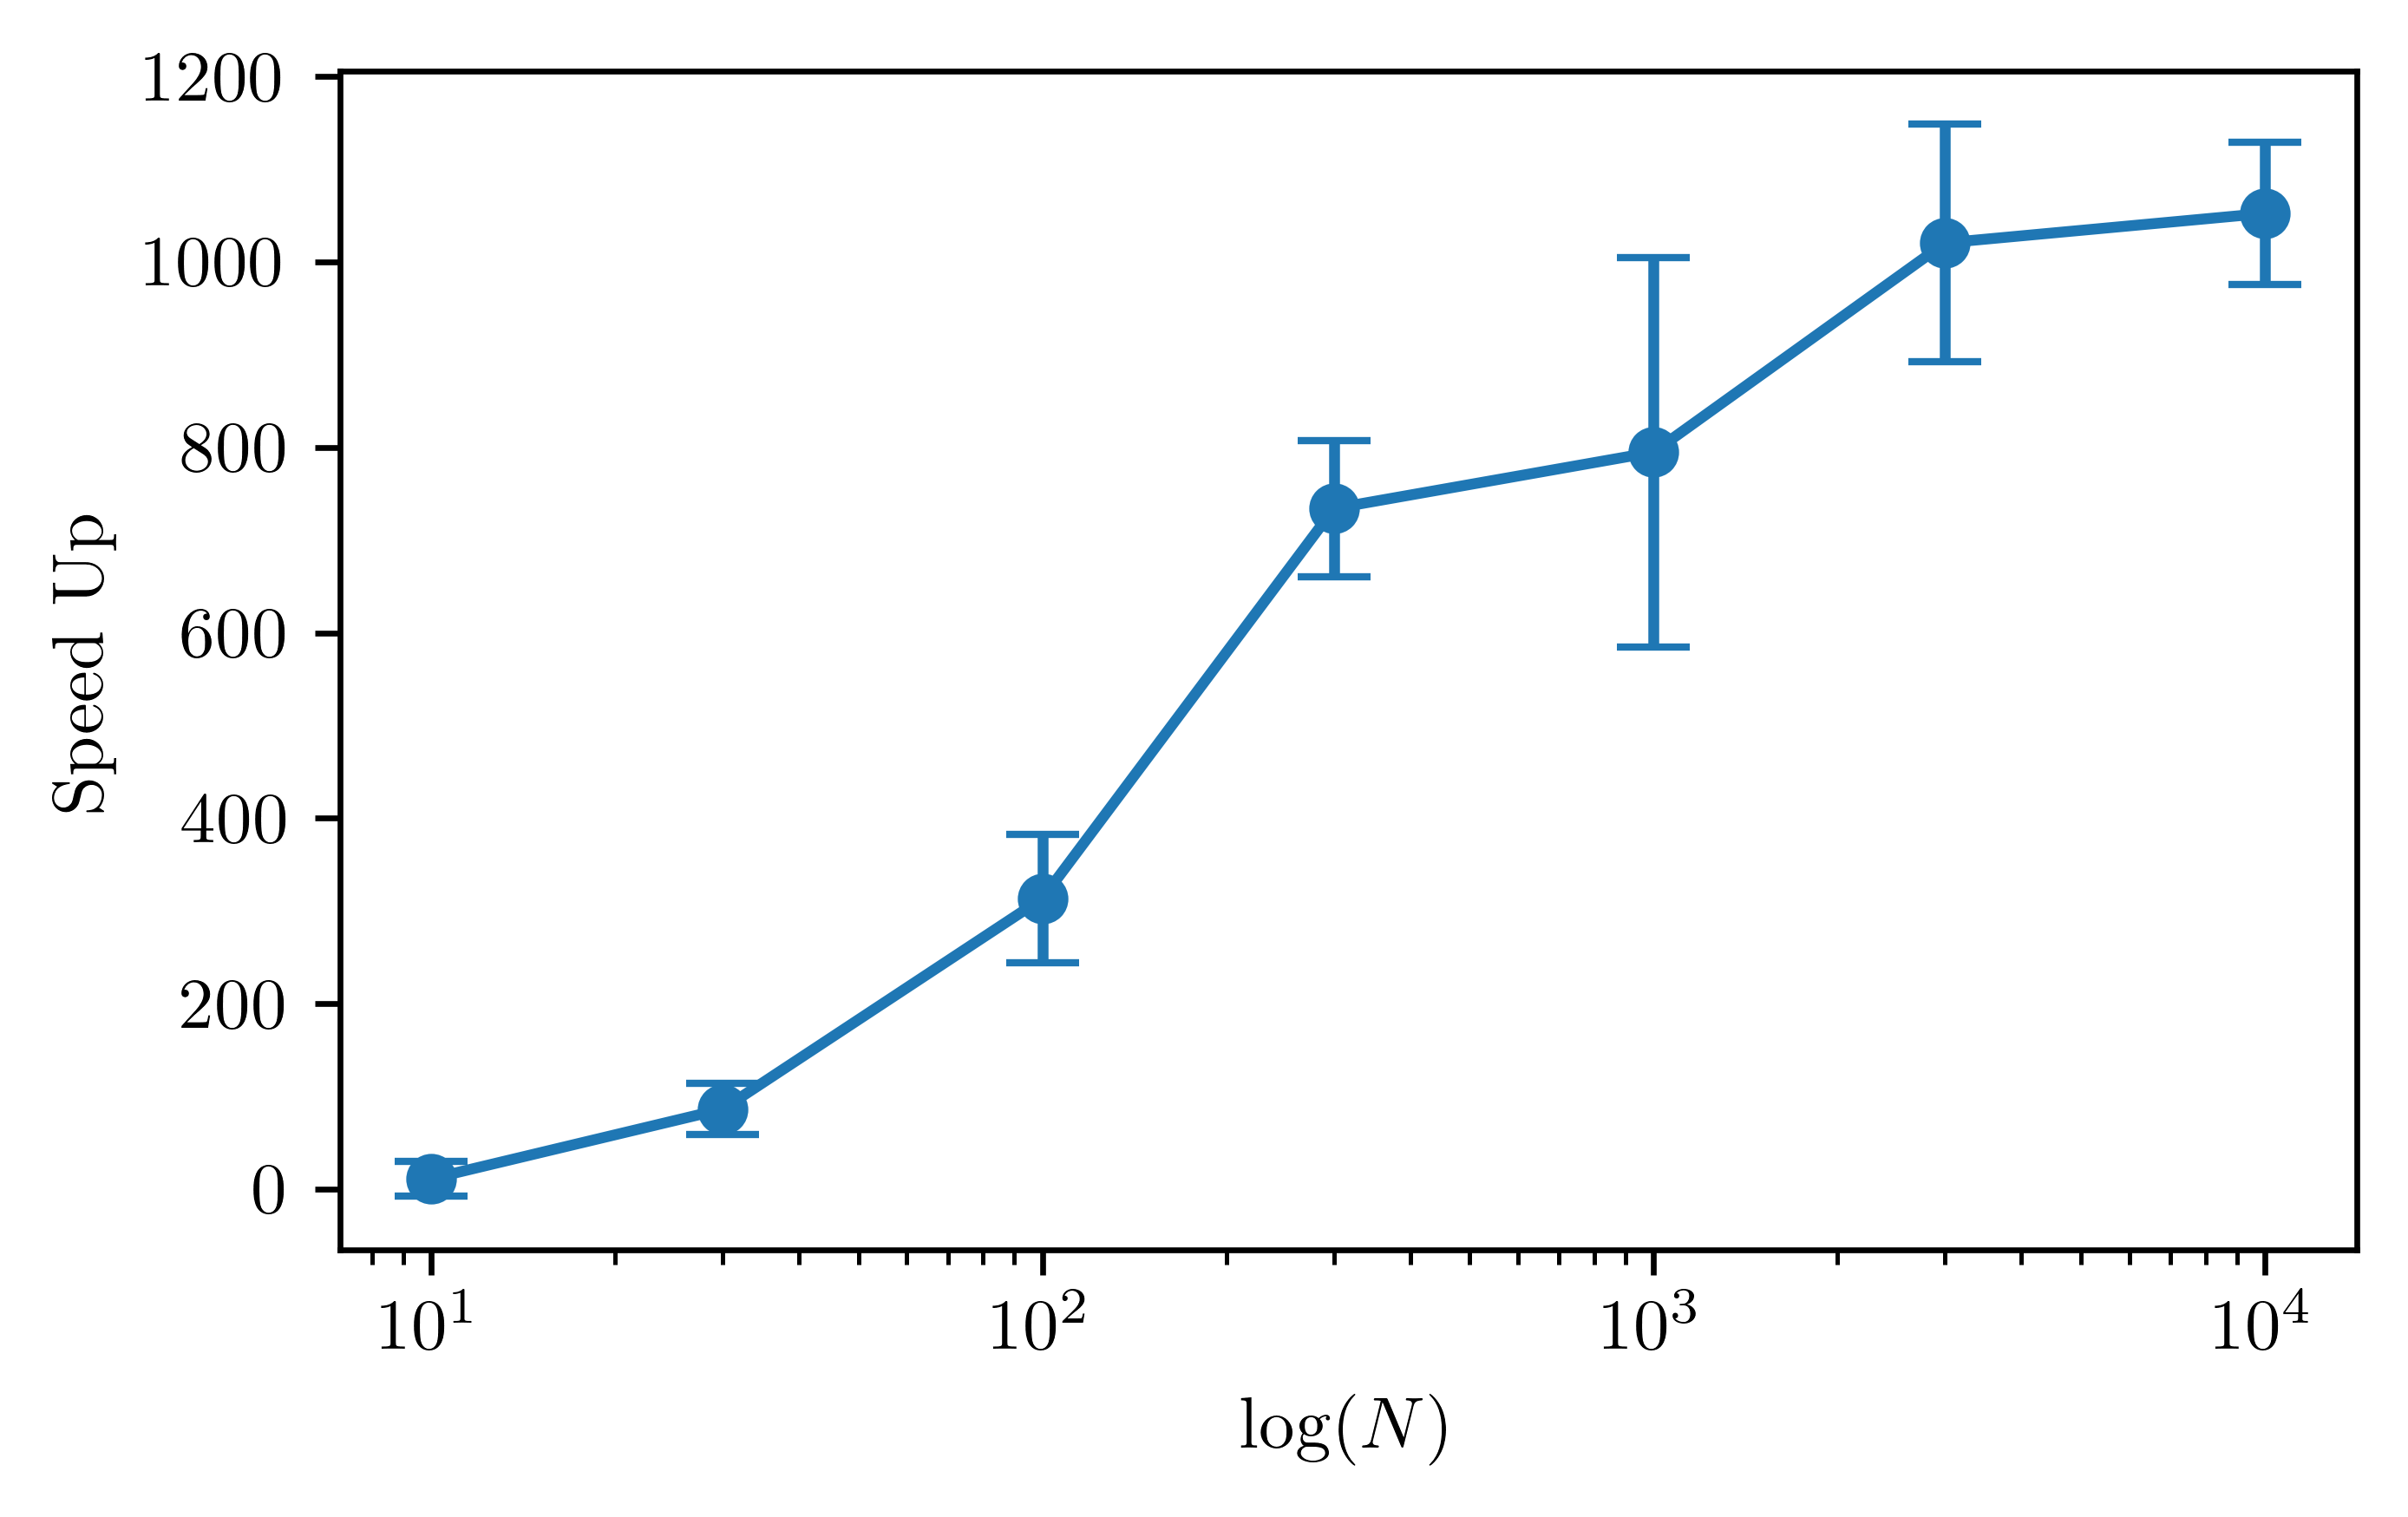
\includegraphics[width=\textwidth]{chapter3/numba_speedup.png}}
  \vspace{0pt}
    \caption{Numpy versus Numpy with Numba benchmarked on an insertion sort. $N$
    refers to the number of integers to sort, and $t$ is the time in seconds taken
    by the implementation to complete the sort.}
    \label{fig:3_1_numba}
\end{figure}


- Estimate cost savings from each parallelization steps
    - multiproc

- Compare experimental results for FMM vs Direct computation as a function of number of particles for the LAPLACE KERNEL!!!!. Justify usage of laplace kernel (paradigm, easy etc.)

- [DIAGRAM] Need to plot the computational complexity.

- Understand cost of computation via pyexafmm compared to state of the art exafmm-t.

- Comment on where the slowness comes from

- no parallelism for operator evaluations

- no parallelism for memory sharing

- lots of copying of same data.

- subtoptimal data formats for m2l - lots of loading.

- suboptimal size of data structures lead to loading from non-cpu memory - which is slow - could be optimized via numexpr etc in the future or more intricate chunking of memory.

- These are justifiable from the time constraints on full-time development.

Figures required:

- KEY RESULT: Benchmarking figure as a function of N-particles
